%% ----------------------------------------------------------------------------
% CVG SA/MA thesis template
%
% Created 03/08/2024 by Tobias Fischer
%% ----------------------------------------------------------------------------
\newpage
\chapter{Experiments}

In this section, we detail experimental methods and results for the generation of the ScanSG dataset and the proposed ScanSG-Transformer model.

\section{Scene Graph Generation}

In order to train a successful 3D-VQA model, we must ensure that its input data, namely generated scene graphs and questions, are of high quality. This section empirically evaluates the impact of different design choices on the quality of the generated scene graphs. We evaluate the design choices for scene graph nodes and edges separately, and choose the best performing parameters for the proposed scene graph dataset. For scene graph nodes, we evaluate the effects of different cropping methods, k-values, and visibility scores on the quality of the node embeddings. For scene graph edges, we evaluate the impact of different threshold values on the quality of the edges in the scene graphs.

All experiments in this section are performed on a smaller subset of the dataset, consisting of 71 scenes, with a total of 2467 objects across scenes. This subset is also used for testing in section XXX.

\subsection{Node quality evaluation}
We evaluate the impact of different cropping methods, k-values and visibility scores on the quality of the generated node CLIP-embeddings. The following paragraphs detail the methods and parameters considered for each of these design choices.

\bigskip \noindent
\textbf{Cropping method:}
We compare the impact of the following cropping methods on node embedding quality (illustrated in Figure XXX):
\begin{enumerate}
    \item A tight, rectangular crop around the object with all background pixels masked out. With this method, the object is centered in the image, and the background is removed. However, CLIP was trained on square images with no background removal. To adapt rectangular crops to CLIP, we use the resizing method described in the original CLIP paper [XXX]: the crop is resized to $224$ in its minimum dimension, and then randomly cropped to a $224 \times 224$ square.
    
    \item A tight, rectangular crop around the object with no further changes. With this method, the object is centered in the image. However, the background is not removed, meaning other surrounding objects could contribute to the embedding, and the image is not square. The rectangular crops are resized as in the original CLIP paper [XXX].
    
    \item A square crop centred around the object, resized to $224 \times 224$. With this method, the crop is square and correctly sized, and no further processing is needed. However, the background is not removed and the non-tight crop means other surrounding objects might contribute to the node embedding.
    
    \item A tight, rectangular crop, resized to $224 \times 224$. With this method, the crop is tight around the object (fewer surrounding objects included in the crop). However, the resized crops distort the image, and CLIP was not trained on distorted images.
\end{enumerate}

\begin{figure}[h!]
    \centering
    \begin{minipage}[b]{0.1\textwidth}
        \centering
        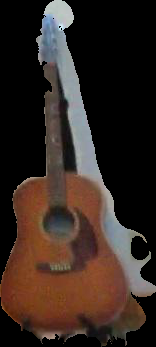
\includegraphics[width=\textwidth]{images/cropping_method_0.png}
        \caption{Caption 1}
    \end{minipage}
    \hspace{1em} % Adjust this to control the horizontal space between images
    \begin{minipage}[b]{0.1\textwidth}
        \centering
        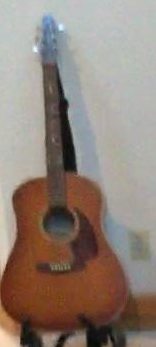
\includegraphics[width=\textwidth]{images/cropping_method_1.png}
        \caption{Caption 2}
    \end{minipage}
    \vspace{0em} % Adjust this to control the vertical space between rows
    \begin{minipage}[b]{0.1\textwidth}
        \centering
        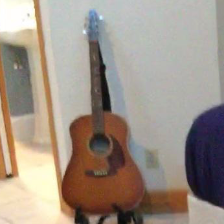
\includegraphics[width=\textwidth]{images/cropping_method_2.png}
        \caption{Caption 3}
    \end{minipage}
    \hspace{1em} % Adjust this to control the horizontal space between images
    \begin{minipage}[b]{0.1\textwidth}
        \centering
        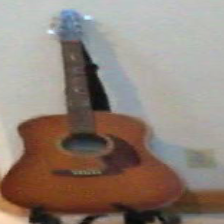
\includegraphics[width=\textwidth]{images/cropping_method_3.png}
        \caption{Caption 4}
    \end{minipage}
    \caption{Overall figure caption}
\end{figure}

\bigskip \noindent
\textbf{k-value:}
We also evaluate the impact of different k-values on the quality of the scene graph nodes. The k-value determines how many images of the object will be considered when generating the scene graph node. A higher value of k could result in a more accurate representation of the object, but could also introduce noise or inconsistencies as different views may have different different embeddings. We not that increasing the k-value highly increases the computational cost. It is therefore important to find the optimal k-value that balances these trade-offs. In this analysis we consider the following k-values: $k=1$, $k=3$, and $k=10$.

\bigskip \noindent
\textbf{Visibility score:}
\begin{enumerate}
    \item multiplied
    \item equal weights, summed
    \item higher weight for pixel score, summed
    \item higher weight for corner score, summed
\end{enumerate}

\textcolor{red}{\textbf{ADD equations + score experiment (compare performance of different scores)}}

To evaluate the comparative quality of these cropping methods and k-values, we perform the following experiment: first, we generate scene graphs using each of the three cropping methods, with $k=1$, $k=3$ and $k=10$ respectively. We therefore have a total of 9 different scene graph node generation methods. Then, we CLIP-embed all the object labels in the scene, and calculate the similarity between the embeddings of the object crops and the embeddings of the object labels. For each object, we select the label with the highest similarity, and compare it to the ground truth label. We calculate the accuracy of the scene graph nodes for each of the 9 methods, and choose the best performing method for the final model.  Note that we only use semantic accuracy (since there is no context-awareness mechanism or learning in this experiment) to evaluate the quality of the scene graph nodes. The semantic accuracy is the percentage of nodes that are embedded closest to their label in the CLIP embedding space. Table XX shows the results of this experiment.

\begin{table}[htbp]
    \centering
    \caption{\textcolor{red}{add title}}
    \begin{tabular}{l|lll|}
    \cline{2-4}
                                                   & \multicolumn{3}{c|}{\textbf{k-value}} \\ \hline
    \multicolumn{1}{|c|}{\textbf{Cropping method}} & 1        & 3       & 10               \\ \hline
    \multicolumn{1}{|l|}{Tight masked crop}        & 49.5     & 50.1    & 52.1             \\
    \multicolumn{1}{|l|}{Tight crop}               & 57.6     & 58.9    & 60.3             \\
    \multicolumn{1}{|l|}{Square crop}              & 57.1     & 58.3    & \textbf{62.2}    \\
    \multicolumn{1}{|l|}{Tight resized crop}       & 56.2     & 57.4    & 60.2             \\ \hline
    \end{tabular}
\end{table}

\textcolor{red}{\textbf{********}}

\bigskip
\noindent
\textbf{CLIP Limitations}
\textcolor{red}{\textbf{Include examples of bad embeddings vs. good embeddings}}

The best score achieved (Table XXX) is fairly low, which indicates that the CLIP-embedding of the object is not very close to the CLIP-embedding of the object label. The experimental examples in Figure XXX provide some insight into why this might be the case.

There are some inherent limitations to the CLIP method, but this is still a good starting point since it allows us to already compare the images of the object with text.

The experiments also highlight the necessity of including some learning into the model, because the CLIP-embedding of the object is not very close to the CLIP-embedding of the object label. And this label task is easier than the question task, as shown in Figure XXX.

\subsection{Edge quality evaluation}

\textcolor{red}{\textbf{Do threshold value experiment: train baseline+gnn on different threshold values and compare performance}}

We train GNN model on the scene graphs with different threshold values for the edges. We evaluate the performance of the model on the test set, and choose the best threshold value for the final sg dataset. We also compare the performance of the model with the best threshold value to the performance of the model with random edges. Table XXX shows the results of this experiment.

Simple GNN model -> show that chosen threshold is better than random edges.
Also show that edges can have a huge impact on the final answer --> must be chosen carefully.

\subsection{Performance on proposed model}
\textcolor{red}{\textbf{Prove that poor design performs worse than good design}}


\newpage
\section{Visual Question Answering Model}

We incrementally build up the proposed model the baseline, adding complexity/degrees of freedom to the model at each step.

Training settings: LR/BS/optimizer/loss function/epochs/dataset/hyperparameters implementation


\begin{table}[h!]
    \centering
    \caption{\textcolor{red}{add title}}
    \begin{tabular}{|l|c|}
    \hline
    \textbf{Model}         & \textbf{Test accuracy} \\ \hline
    Baseline               & 28.1                   \\ \hline
    Baseline + GNN         & \multicolumn{1}{l|}{}  \\ \hline
    ScanSG-GNN             & 25.5                   \\ \hline
    ScanSG-Transformer     & \textbf{46.4}          \\ \hline
    GraphVQA (pre-trained) & \multicolumn{1}{l|}{}  \\ \hline
    \end{tabular}
\end{table}

\textcolor{red}{\textbf{Complete table}}


1) start from the baseline model --> accuracy is quite low because 1-no edge information/context awareness 2-no learning (relies on static, pre-computed embeddings and cannot adapt to the data). Object selection block: CLIP(question) vs CLIP(answer) --> similarity with static embeddings does not work well - we show that CLIP(question) does not really capture the same meaning as CLIP(answer)

2) add edge information --> GNN model to propagate edge information / give the scene representation some context awareness - each node inherits information from its neighbouring nodes. but this doesnt work well because we still use the cosine similarity of a dynamic embedding and a static embedding (from question), but while the questions might have the same answer their embeddings could be very different. training GNN-only model incentivises the model to make the object embeddings  similar to the question embeddings from the training set but these could be very different. this means the model 1) receives a lot of noise in the form of the question embeddings and 2) does not learn to adapt to the data.

3) add learning to similarity score and text embedding --> proposed model

4) use transformer instead of GNN for scene encoding (performs better but doesnt learn from graph structure but rather language priors...), two scenes with objects in different positions would have the same scene representation.


\textcolor{red}{\textbf{Show results for other evaluation metrics: EM@5, EM@10, loss}}


\textcolor{red}{\textbf{Include plot which shows overfitting problem}}
Overall, there is a overfitting problem. This can either be due to the model (model is too complex, not regularized enough, ...) or the data (not enough data, data is too hard, ...).

Model changes to attempt to overcome this, we report the results of the best performing model with the following changes: 
normalization
dropout
L2 regularization
changing loss function, ...

\textcolor{red}{\textbf{do the following experiments:}}
downsizing embedding
word-level embedding (rather than last layer)